\documentclass[12pt]{article}
% \documentclass[conference]{IEEEtran}

% Packages
% Packages

% \usepackage{fancyhdr} % Required for custom headers
% \usepackage{lastpage} % Required to determine the last page for the footer
% \usepackage{extramarks} % Required for headers and footers
% \usepackage[usenames,dvipsnames]{color} % Required for custom colors
\usepackage{graphicx} % Required to insert images
% \usepackage{listings} % Required for insertion of code
% \usepackage{courier} % Required for the courier font
% \usepackage{dsfont} % For special math characters
% \usepackage{verbatim}

%\usepackage{amsmath, amssymb, bm} % For matrix notation
\usepackage[english]{babel}
\usepackage[paperwidth=8.5in,paperheight=11in,margin=1.0in]{geometry}
\usepackage{listings}
\usepackage{hyperref}
%\usepackage[cmex10]{amsmath, bm}
\usepackage{amsmath, bm}
\usepackage{blkarray}








% formatting
\pdfcompresslevel0

\lstset{ columns=flexible, breaklines=true, basicstyle=\small\ttfamily}
\setcounter{MaxMatrixCols}{20}
\linespread{1.3} %1.5x line spacing




\begin{document}
\title{Predicting Salaries From Job Descriptions}

\author{
Elijah Bernstein-Cooper, Ben Conrad, Ahmed Saif
}
\maketitle

%NB: Double ticks do not work for apostrophes, look at the output before changing all.  They do work for the first quotation mark.


% ------------------------------------------------------------------------------
\section{Introduction}
% ------------------------------------------------------------------------------

    Under the context of natural language processing, this lab explores the
    relation between job descriptions and salaries.  This topic was the focus
    of a \href{http://www.kaggle.com/c/job-salary-prediction}{Kaggle}
    competition whose sponsor, Adzuna, had a database of job listings of which
    only half provided salary information (the winner received \$3000).  As
    applicants will more likely apply to descriptions that give a salary,
    Adzuna's placement rate (and hence Adzuna's) is improved if they can provide
    an estimated salary for those descriptions that did not originally include
    one. The employee recruiting business is structured so that Adzuna
    generally can't directly ask the companies to provide salary estimates.
    This is challenging from the legal standpoint, as grossly incorrect	
    salaries may expose Adzuna to claims from applicants and companies, and
    applicant experience, since Adzuna's estimates must seem plausible to
    applicants before they will be willing to spend the time applying.

    While Adzuna could manually estimate these salaries, scalability encourages
    throwing computers at the problem.  In this lab we will be using Adzuna's
    job description and salary datasets, divided into training and test sets.
    These descriptions vary in word count, industry, employment level, and
    company location, while the salaries are the mean of the provided salary
    range.  The variability in description content leads to notoriously sparse
    matrices, so we will be interested in the tradeoffs of various feature
    descriptors.  The naive approach to this problem is to count the
    occurrences of individual words and associate them to salaries; here each
    word is a feature and as there are many descriptive words the resulting
    matrices will be sparse.  Other feature choices may be individual word
    length, occurrences of word pairs or triplets (i.e. ``technical
    communication"), n-grams (sequences of n characters), and many others. It
    is common to ignore stop words like ``the",``a",``it",``you",``we", etc.
    because they add little information.

% ------------------------------------------------------------------------------
\section{Warm-Up}
% ------------------------------------------------------------------------------

    Our goal in the warm-up is to use two job descriptions with known
    salaries to predict the salary of another job given the description. Here
    are two examples from the dataset: 
    
    \begin{lstlisting}

        Engineering Systems Analyst Dorking Surrey Salary ****K Our client is
        located in Dorking, Surrey and are looking for Engineering Systems
        Analyst our client provides specialist software development Keywords
        Mathematical Modelling, Risk Analysis, System Modelling, Optimisation,
        MISER, PIONEEER Engineering Systems Analyst Dorking Surrey Salary ****K

    \end{lstlisting}

    with a salary of \$25,000 and 

    \begin{lstlisting}

        A subsea engineering company is looking for an experienced Subsea Cable
        Engineer who will be responsible for providing all issues related to
        cables. They will need someone who has at least 1015 years of subsea
        cable engineering experience with significant experience within
        offshore oil and gas industries. The qualified candidate will be
        responsible for developing new modelling methods for FEA and CFD. You
        will also be providing technical leadership to all staff therefore you
        must be an expert in problem solving and risk assessments. You must
        also be proactive and must have strong interpersonal skills. You must
        be a Chartered Engineer or working towards it the qualification. The
        company offers an extremely competitive salary, health care plan,
        training, professional membership sponsorship, and relocation package
    
    \end{lstlisting} having a salary of \$85,000.

    One method to predict the salary from another description is least squares
    estimation.  Least squares estimation can be thought of as an optimization
    problem which aims to minimize the error estimated and measured data.  In
    our case, we want to predict salaries from the words contained in the job
    descriptions.  For now, let's consider only occurrences of ``analyse" in
    the description.  If you plot the number of occurrences against the job
    salary, you might produce something like
    
    \begin{center}
    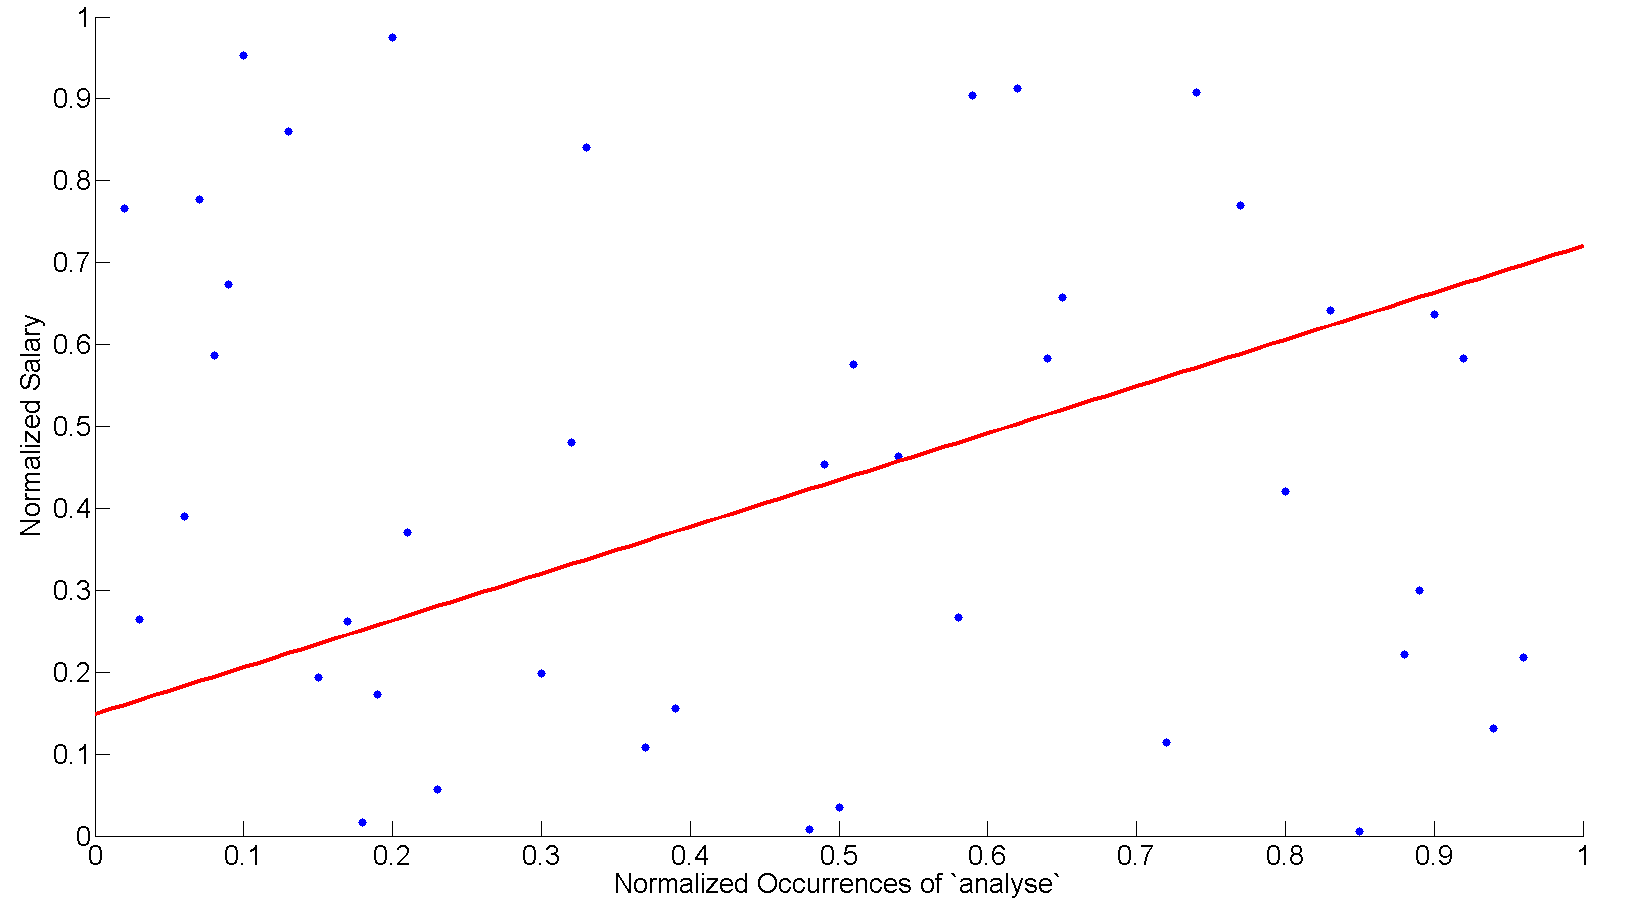
\includegraphics[width=\linewidth]{figLSE}
    \end{center}
    
    In solving the least squared problem, we're looking for the line which
    passes nearest to all of the points, as measured by the Euclidean distance,
    or

    \begin{equation}
    error = \sqrt{ (x_i - x_L)^2 + (y_i - y_L)^2} 
    \end{equation}
 
    If we considered two words, say ``analyse" and ``qualified", we would now
    have a 3D space to find our least squared solution with one axis being
    occurrences of ``analyse," another ``qualified," and the third the salary.
    Here, our solution will be a plane that slices the 3D space; adding more
    words - or features as they're more generally described - increases the
    dimensionality of this space, and our solution becomes a hyperplane.  In
    all cases, we want to minimize the distance from all of the data points to
    the lower-dimensional estimate.
    
    We would like to determine the words that best predict salary, or even
    better the frequency of the words which best predict salary. Here we show
    the 11 most common words for each description:

    \begin{center}
    \begin{minipage}[t]{.4\textwidth}
    Description 1
    \newline
    \newline
        \begin{tabular}{l|c}
            ****k & 2 \\
            analysis & 1\\
            analyst & 3\\
            and & 1\\
            are & 1\\
            client & 2\\
            development & 1\\
            dorking & 3\\
            engineering & 3\\
            for & 1\\
            in & 1
        \end{tabular}
    \end{minipage}
    \begin{minipage}[t]{.4\textwidth}
    Description 2
    \newline
    \newline
        \begin{tabular}{l|c}
            1015 & 1 \\
            a & 2 \\
            all & 2 \\
            also & 2\\
            an & 3 \\
            and & 5 \\
            assessments & 1 \\
            at & 1 \\
            be & 6 \\
            cable & 2 \\
            cables & 1
        \end{tabular}
    \end{minipage}
    \end{center}

    We can collect these word counts into matrix $\bm{A}$, and the salaries
    into vector $\bm{b}$. $\bm{A}$ will have 2 rows, one for each
    description and as many columns as there are unique words between the two
    descriptions. $\bm{b}$ will have 2 rows, one salary for each description,
    and one column. $\bm{A}$ and $\bm{b}$ will look like the following

    \begin{equation*}
        \bm{A} = 
        \begin{bmatrix}
           2 & 0 & 0 & 0 & 0 & 0 & 1 & 3 & 1 & 1\cdots\\
	0 & 1 & 2 & 2 & 2 & 3 & 0 & 0 & 5 & 0\cdots
        \end{bmatrix}
    \end{equation*}
	
    \begin{equation*}
        \bm{b} = 
        \begin{bmatrix}
        25000\\
        85000
        \end{bmatrix}
    \end{equation*}
    with the first 2 corresponding to the two occurrences of `****k' in the first descripton and the later 1, 5 column to occurrences of `and' in both descriptions.


    We can then set up our problem as 
    \begin{equation}\label{eq:linsolve}
        \bm{b} = \bm{Ax}
    \end{equation}

    \noindent where $\bm{x}$ contains the weights (importance) of each word in
    predicting the salary of the job. We can find a solution for $\bm{x}$,
    $\bm{\hat{x}}$, by minimizing the residual errors between $\bm{b}$ and
    $\bm{Ax}$.  This is the same as minimizing the sum of squared residuals,

    \begin{equation}
        \|\bm{b} - \bm{Ax}\|^2_2
    \end{equation}

    \noindent This optimization has a well-known solution for $\bm{\hat{x}}$
    \begin{equation}
        \bm{\hat{x}} = (\bm{A}^{T}\bm{A})^{-1}\bm{A}^T\bm{b}
    \end{equation}
    when $\bm{A}$ is positive semidefinite and, therefore, invertible.
    
    In cases when $\bm{A}$ is not positive semidefinite, as in the $\bm{A}$
    derived from the word counts above, we can use the right psuedo-inverse of
    $\bm{A}$.  In Matlab this is 
    
    \begin{equation} 
        \bm{\hat{x}} = \texttt{pinv}(\bm{A})*\bm{b}
    \end{equation}

    The least squares solution to this problem is

    \begin{equation*}
        \bm{\hat{x}} = 
        \begin{blockarray}{[c] l}
            1819.6517 & ``be"           \text{ from } [0, 6] \\
            1730.9558 & ``and"          \text{ from } [1, 5] \\
            1427.6805 & ``for"          \text{ from } [1, 4] \\
            1250.2887 & ``engineering"  \text{ from } [3, 2] \\
            1213.1011 & ``must"         \text{ from } [0, 4] \\
            1213.1011 & ``will"         \text{ from } [0, 4] \\
            1213.1011 & ``you"          \text{ from } [0, 4] \\
            909.8258 & ``an"            \text{ from } [0, 3] \\
            909.8258 & ``subsea"        \text{ from } [0, 3] \\
            909.8258 & ``the"           \text{ from } [0, 3] \\
            732.4341 & ``modelling"     \text{ from } [2, 1] \\
            \vdots & \hspace{1cm}\vdots
        \end{blockarray}
    \end{equation*}

    The bracketed numbers give the number of occurrences of that word in each
    of the descriptions; with only two samples it should not be surprising that
    the most heavily-weighted words are unique to each description.  But notice
    how some words are identically-weighted and that from these 11 `most
    important' words, few of them are highly descriptive.
    
    % --------------------------------------------------------------------------
    % Activity 
    % --------------------------------------------------------------------------
    \begin{center} 
        
        \fbox{\begin{minipage}{35em} {\bf \large Activity 1} \\ Construct the
                above $\bm{A}$ and $\bm{b}$ matrices using the 1$^{\rm st}$ and
                2$^{\rm nd}$ descriptions in \texttt{activity1.mat}.
                $\bm{A}$ should be a 2$\times m$ matrix
                where $m$ is the number of unique words between the two
                descriptions.  $\bm{b}$ should be a 2$\times$1 matrix. Can you
                reproduce the above solution for $\bm{\hat{x}}$? Report on the
                uniqueness of the solution for $\bm{\hat{x}}$ in this problem.
                Support your conclusion.\\
            
            The following commands may be helpful:
            \begin{center}
                \texttt{word = strrep(`word',`charactersToReplace',`replaceThemWith')} \\
                \texttt{parts = strsplit('sentence')}\\
                \texttt{lowercase = lower('UpperCase')}\\
                \texttt{uwords = unique(wordArray)}\\
                \texttt{sortedArray = sort(unsortedArray)}\\
            \end{center}
            \end{minipage}
        }
        
    \end{center}
    % --------------------------------------------------------------------------
    % --------------------------------------------------------------------------
    
    Next we wish to predict the salary of another description using our
    $\bm{\hat{x}}$. 

    \begin{lstlisting}
        Our client is part of an international hotel chain that require an
        experienced Cluster Revenue Manager to be based in Hertfordshire. The
        Cluster Revenue Manager will drive and influence revenue for three to
        four hotels. As Cluster Revenue Manager you will maximise revenue,
        market share and profits for multiple hotels through the strategic
        coordination of revenue management processes and procedures. The
        Cluster Revenue Manager will drive the continued development and growth
        of customer service standards, revenue and profits from multiple hotels
        and to deliver the company's mission relating to profit, people,
        customer and quality. You will currently be a Cluster Revenue Manager
        or a Regional/ Area Revenue Manager looking after a minimum of two
        propertys or a Revenue Manager in a large unit managing both rooms and
        conference space. This job was originally posted as
        www.caterer.com/JobSeeking/ClusterRevenueManager_job****
    \end{lstlisting} having a salary of \$45,000.
    
    % --------------------------------------------------------------------------
    % Activity 
    % --------------------------------------------------------------------------
    \begin{center} 
        
        \fbox{\begin{minipage}{35em}

            {\bf \large Activity 2} \\
            Use your solution for $\bm{\hat{x}}$ in Activity 1 to estimate the
            salary of the third description in the activity 1 data.  
            Since $\bm{\hat{x}}$ is a weighting of words
            from the first two descriptions, ignore any words that are unique
            to the third description.
            \end{minipage}
        }
        
    \end{center}
    % --------------------------------------------------------------------------
    % --------------------------------------------------------------------------

    We now construct the matrix $\bm{A}$ for this description. This matrix will
    only contain frequencies of words that were present in the previous two
    descriptions, so many words in this new description will be left out. We
    can then use our weights for best predicting words, $\bm{\hat{x}}$ to
    estimate the salary of the job for this new description, now contained in
    the matrix $\bm{b}$. Our estimated salary will be stored in $\bm{\hat{b}}$,
    which we estimate from Equation~\ref{eq:linsolve}. \\

    The estimated salary is \$3,032.80. About \$41,967 different from the true
    salary associated with the job. Would Adzuna likely use this technique of
    linear least squares? Consider how populated our $\bm{A}$ matrix is for the
    third description. Is the matrix well-populated or sparsely-populated?
    Based on your intuition, are all of the words in $\bm{\hat{x}}$ likely to
    be good predictors of salary? How might paring down the keywords in our
    data matrix benefit us? In the following sections we will introduce ways to
    include many more descriptions in our analysis, and derive more accurate
    predictors of a salary based on the description.

% ------------------------------------------------------------------------------
\section{Larger Datasets and Regularized Least Squares}
% ------------------------------------------------------------------------------

    We have seen how a least squares fit to only two descriptions chooses the
    most common word in the job description associated with the highest salary
    to best predict a higher salary. Predicting the word ``be'' goes against
    intuition. In the warm-up activity, our least squares fit was
    underdetermined, meaning that there were more variables than equations.
    With more descriptions we may be able to have more equations than
    variables, the overdetermined case, which has a unique solution which will
    likely be more intuitive.

    % --------------------------------------------------------------------------
    % Activity 
    % --------------------------------------------------------------------------
    \begin{center} 
        
        \fbox{\begin{minipage}{35em}

            {\bf \large Activity 3} \\

            Following the same method as in the warm-up, describe how the
            frequency matrix will change with added descriptions. If we include
            every word from each of the descriptions in our frequency matrix,
            is it likely that the number of salaries will be greater than the
            number of words in the frequency matrix? Describe how the
            computation time scales with the size of the frequency matrix. Is
            it practical to include every word from each description in the
            frequency matrix?

            \end{minipage}
        }
        
    \end{center}
    % --------------------------------------------------------------------------
    % --------------------------------------------------------------------------

    Lets consider a more realistic example where we are provided 10
    descriptions from an individual industry sector each with a salary
    provided. We will be working with the industry ``Customer Services Jobs''. 
    
    % --------------------------------------------------------------------------
    % Activity 
    % --------------------------------------------------------------------------
    \begin{center} 
        
        \fbox{\begin{minipage}{35em}

            {\bf \large Activity 4} \\
            
            Load the activity data, activity$\_$train.mat and
            activity$\_$train.mat. With each data set construct a frequency
            matrix of words, excluding common words you are confident will not
            be important to a description's salary. Derive a linear least
            squares solution for $\hat{\bm{x}}$ in Equation~\ref{eq:linsolve}
            with the first 10 descriptions in the training set. Predict the
            salaries of the first 10 descriptions in the test set. Report the
            $L_2$ norm of the difference between the true salaries and
            predicted salaries for the test set. Report the word which is best
            able to predict the salary of a description. State whether this
            problem is over determined or under determined.

            \end{minipage}
        }
        
    \end{center}
    % --------------------------------------------------------------------------
    % --------------------------------------------------------------------------

    We can see again that the least squares problem is again not unique. One
    way to derive a unique solution in an under determined linear equation is
    to use regularized least squares. This is similar to least squares, but
    with an additional smoothing term in the minimization

    \begin{equation}
        \min_x \|\bm{b} - \bm{Ax}\|_2^2 + \lambda\|\bm{x}\|_2^2
    \end{equation}

    \noindent where $\lambda > 0$. $\lambda$ is the smoothing parameter. Larger
    $\lambda$ values favor smaller $L_2$ norms, while small $\lambda$ values
    return the minimization to linear least squares.  Essentially
    regularization allows for a unique solution that can be smoothly varying,
    and not sensitive to small changes in the frequency matrix. The solution to
    regularized least squares is given by

    \begin{equation}
        \bm{\hat{x}} = (\bm{A}^{T}\bm{A} + \lambda \bm{I})^{-1}\bm{A}^T\bm{b}
    \end{equation}

    \noindent where $\bm{I}$ is the identity matrix. We will explore a similar
    regularization in the next section which will help us minimize the number
    of words that we include our solution.

% ------------------------------------------------------------------------------
\section{The Lasso Method}
% ------------------------------------------------------------------------------

    One of the issues with predicting a job salary is choosing what key words
    we should use to predict them. As we have seen, the number of words even
    for small datasets used to construct frequency matrices and weighting
    solutions quickly grows out of hand. Fortunately, there are ways of
    automatically choosing what words we should choose in predicting the salary
    for the ads. One such method is the Lasso method, another form of
    regularization similar to regularized least squares. The Lasso method
    attempts to solve the following equation

    \begin{equation}
        \min_x \|\bm{b} - \bm{Ax}\|_2^2 + \lambda\|\bm{x}\|_1
    \end{equation}

    \noindent which is minimizing the least square solution along with the
    absolute values word weights. By making $\lambda$ large you are making
    $\bm{x}$, the number of words you predict salaries with, small. Smaller
    $\lambda$ values correspond to using all words, or back to the linear least
    squares minimization. This form of regularization removes words with low
    frequencies thus removing the sparsity in the matrix, i.e., removing mostly
    zero word occurrences in lots of examples. 

    The implementation of the Lasso method is not so trivial however. There is
    no closed-form solution to solving the Lasso method. however there are good
    approximations that derive solutions quickly. The following describes the
    pseudo-code for implementing the Lasso method:

    \begin{minipage}{35em}

        \begin{enumerate}
            
            \item Initialize two weight vectors for the frequency matrices,
                $\hat{\bm{x}}$ and $\hat{\bm{x}}^\prime$, consisting of zeros,
                with lengths equal to the number of unique words in all
                descriptions.

            \item Take singular value decomposition of frequency matrix
                $\bm{A}$ by \texttt{[T, S, V] = svd(A)}

            \item Initialize $\alpha$ to largest singular value of
                decomposition of $\bm{A}$ 1/max($\bm{S}$)

            \item Set $\Delta$, the 2-norm of the difference between
                $\hat{\bm{x}}$ and $\hat{\bm{x}}^\prime$ to a large value.
                
            \item While $\Delta$ is larger than the tolerance and the iteration
                number is less than the maximum iteration do

                \begin{enumerate}

                    \item Set $\hat{\bm{x}}$ = $\hat{\bm{x}}^\prime$
                    
                    \item Set $\bm{Y}$ = $\hat{\bm{x}}$ + $\alpha$ $\bm{A}^T
                        (\bm{b - A} \hat{\bm{x}}$)

                    \item Set $\hat{\bm{x}}^\prime$ = sign($\bm{Y}$)
                        $\max(|\bm{Y}| - \alpha \lambda$, 0)

                    \item Increase the iteration number

                    \item Set $\Delta$ = $\|\hat{\bm{x}}$ -
                        $\hat{\bm{x}}^\prime\|$

                \end{enumerate}

            \item Return $\hat{\bm{x}}$ as the predictor.

        \end{enumerate}
    \end{minipage}

    % --------------------------------------------------------------------------
    % Activity 
    % --------------------------------------------------------------------------
    \begin{center} 
        
        \fbox{\begin{minipage}{35em}
Add some visualization like \texttt{[\~,xinds] = sort(abs(xhat),'descend');}
\texttt{plot(1:length(xhat),xinds,'.')}

            {\bf \large Activity 5a} \\
    
            Construct a function for the Lasso method. Perform the Lasso method
            on all 100 descriptions using the datasets
            \texttt{activity$\_$test.mat} and \texttt{activity$\_$train.mat}.
            Set $\lambda$ = 10. The resulting $\hat{\bm{x}}$ value should be
            all zeros except for 2 values, corresponding to the predicting
            words ``experience'' and ``client''. Predict the salaries of the
            test data using the training data. Report the 2-norm of the
            difference between the predicted and the true salaries. Make a
            histogram of the residuals between the predicted and the true
            salaries.\\
            
            {\bf \large Activity 5b} \\

            Perform the Lasso method with different values of $\lambda$ = 10,
            5, 2, 1. Record the number of important words, (words with non-zero
            weights), the important words, and the 2-norm of the difference
            between the true and predicted salaries. Summarize the results in a
            table. Make a histogram of the residuals between the predicted and
            the true salaries for each of the $\lambda$ values as well.\\
            
            {\bf \large Activity 5c} \\

            Experiment with the Lasso method using smaller values of
            $\lambda$.  What $\lambda$ value do you think keeps the number of
            words reasonable while still including enough words in the weight
            matrix to accurately predict the salary? This can be an art, there
            is not a correct answer. 

            \end{minipage}
        }
        
    \end{center}
    % --------------------------------------------------------------------------
    % --------------------------------------------------------------------------


\section{Using the Results}
We've seen that accurate salary prediction is a function of the algorithm and the size of the training set, and while there are many additional improvements, let's conclude by exploring some results of this analysis.

Recall that the basic form of the least squares problem is $\bm{b = Ax}$.  We
formed $\bm{A}$ by counting the number of occurrences of each word in the job
description and placed the corresponding salaries in $\bm{b}$.  $\bm{A}$ can be
viewed as a mapping from word-weight space (home of $\bm{x}$) to salary space,
with the reverse mapping coming from $\bm{A}$'s inverse.  $\bm{x}$ was then the
weight or descriptiveness of each word - how useful its number of occurrences
were in predicting the correct salary.

$\bm{A}$ is a linear operator, so if a particular applicant wants to make
\$50,000, we can determine which words they should look for when reading
descriptions by computing $\bm{sum(}\texttt{pinv}\bm{(A)50000,2)}$.
If the
applicant includes these descriptive words in their objective statement or
elsewhere in their resume, it seems reasonable to expect that their application
will be successful (though this is a different - if similar - problem).  We can
also use the $\bm{A}$ and $\bm{x}$ computed from the training data to analyze a
resume and suggest what salary their resume implicitly seeks.

    % --------------------------------------------------------------------------
    % Activity 
    % --------------------------------------------------------------------------
    \begin{center} 
        
    \fbox{
	\begin{minipage}{35em}
	{\bf \large Activity 6a} \\
The loaded data also contains the {Modern Major General's song} and a sample undergraduate electrical engineering resume as \texttt{majorGen} and \texttt{elecGrad}.
Predict how much the Major General and EE grad would make if applying to jobs similar to those in the training set.\\

	{\bf \large Activity 6b} \\
The salaries fall substantially below the poverty line in any country; why is this the case?
Compare the most important keywords against those contained in \texttt{majorGen} and \texttt{elecGrad}; it may help to consider how the predicted salary is computed.
	\end{minipage}
     }
\end{center}
    % --------------------------------------------------------------------------
    % --------------------------------------------------------------------------

It is beyond the scope of this lab to consider other machine learning strategies that may be more successful and/or faster in solving this problem, but having reached this point it's worth commenting that this method is easy to understand.
That is, it's easy to inspect and debug and can give good results without heavily relying on statistical concepts.
Achieving good results requires some tuning; even though the test salary prediction error was below [final error], it had difficult predicting the Major General and EE grad salaries.
This difference is due to the differing writing styles between the job descriptions, Major General's song, and EE grad resume.


\end{document}




